\chapter{Opis projektnog zadatka}

\textbf{\textit{Uvod}}\\

Cilj projekta "Medicinska rehabilitacija" je razvoj programske podrške za stvaranje istoimene web aplikacije koja će omogućiti korisnicima jednostavno naručivanje za fizikalnu terapiju i medicinsku rehabilitaciju. Korisnici u našem slučaju su pacijenti koji su se ozlijedili te trebaju stručnu pomoć. Zadatak nam je omogućiti intuitivno korisničko sučelje kako bi olakšali korištenje aplikacije pacijentima, ali i zdravstvenim djelatnicima.

Glavna motivacija bila nam je modernizacija hrvatskog zdravstva. Vjerujemo kako pacijentima nije drago zvati mobitelom svoje doktore znajući da su pretrpani poslom, a također im je dosta čekanje na odgovor zdravstvenog djelatnika kada im se pošalje mail. S druge strane nije ni zdravstvenim djelatnicima lako odgovarati na sve te silne poruke. Ovom aplikacijom bismo omogućili pacijentima da biraju dostupan termin koji njima najbolje odgovara, a doktore poštedili dodatnog posla.

Između ostalog ova bi aplikacija omogućivala liječnicima praćenje poboljšanja zdravstvenog stanja pacijenata. Ako se pacijenti prvi puta naručuju za terapiju potrebna je registracija, a svaki sljedeći put je nužna prijava u sustav. Za registraciju potrebni su sljedeći podaci: 
\begin{packed_item}
	\item \textit{ime i prezime}
	\item \textit{korisničko ime}
	\item \textit{lozinka}
	\item \textit{e-mail adresa}
	\item \textit{OIB}
	\item \textit{spol}
	\item \textit{datum rođenja}
\end{packed_item}

Administrator gornje podatke mora verificirati iz središnjeg informacijskog sustava zdravstvene zaštite. Pacijenti prilikom zakazivanja termina moraju navesti vrstu i opis svojih oboljenja, zahtijevani postupak liječenja te vrijeme koje bi im odgovaralo za termin. Ako se ne radi o prvom dolasku u ustanovu zahtijeva se i prikaz reference na već obavljeni postupak u toj ustanovi. Zdravstveni djelatnici dodjeljuju termine tako da vode brigu o ukupnom kapacitetu opreme/uređaja, kapacitetu prostorija, osobnim mogućnostima te trajanju svakog zahvata. Nakon dobivenog termina pacijentu dolazi e-pošta sa terminom te ostalim dodatnim informacijama. U slučaju neočekivanih promjena djelatnik može kontaktirati bolesnika putem e-pošte. Radno vrijeme ustanove u kojoj se provodi rehabilitacija je svakim radnim danom od 8 do 20 sati. Ustanova ima pravo odrediti određene slobodne dane na temelju blagdana ili praznika.\\

\textbf{\textit{Primjer sličnog rješenja}}\\

Primjer sličnog rješenja je web aplikacija "YouCanBookMe". To je aplikacija koja omogućuje čovjeku koji prima klijente da postavi svoje termine u kojima je dostupan, a klijentima odabir termina koji njima odgovaraju. Sličnost s našim sustavom je ta što će zdravstveni djelatnik moći određivati u kojim terminima je dostupan, a klijent će moći odabrati jedan od tih dostupnih termina. Ova web aplikacije je općenamjenska, dok naša ima primjenu u medicini. 

\begin{figure}[H]
	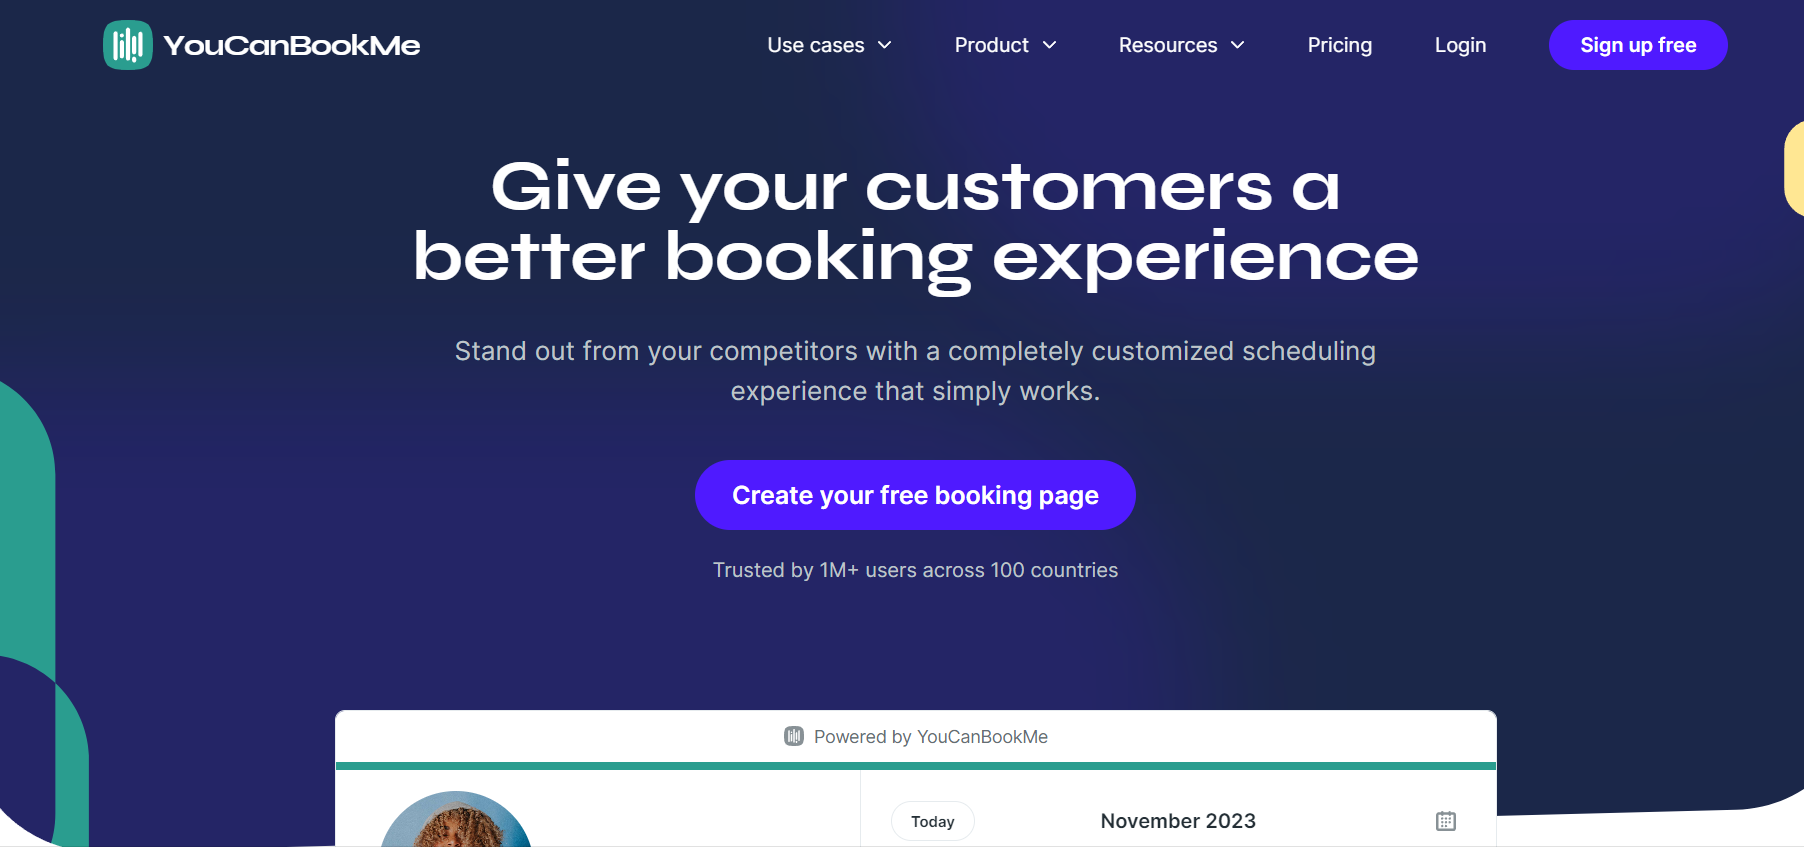
\includegraphics[scale=0.36]{slike/YouCanBookMe-Naslovna.PNG} %veličina slike u odnosu na originalnu datoteku i pozicija slike
	\centering
	\caption{Naslovna stranica "YouCanBookMe" aplikacije}
	\label{fig:promjene}
\end{figure}

Registracija je omogućena putem upisivanja email adrese, lozinke i ostalih podataka. Neki od važnijih preostalih podataka su ime i prezime osobe. Sigurnost podataka ostvarena je tako da korisnik na svoj email dobiva sigurnosni kod koji treba upisati kako bi uspješno bio registriran. 

Prijava u sustav je omogućena tek nakon registracije korisnika, a potrebni podaci koje trebamo upisati su email i lozinka. Izgled stranice za prijavu je vrlo sličan izgledu stranice za registraciju.

\begin{figure}[H]
	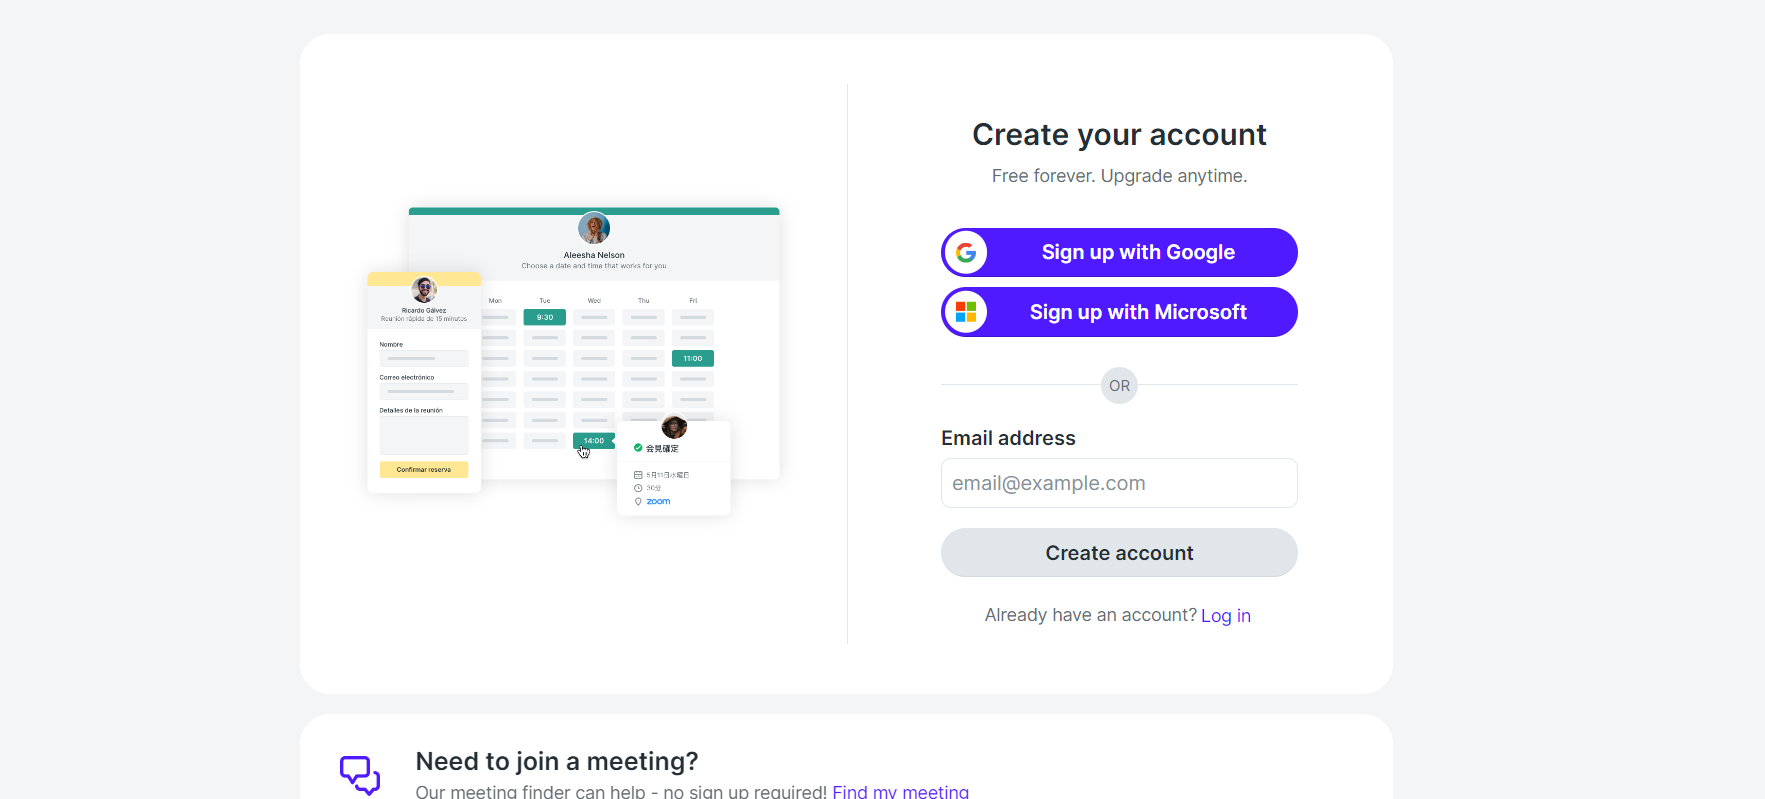
\includegraphics[scale=0.4]{slike/YouCanBookMe-Registracija1.PNG} %veličina slike u odnosu na originalnu datoteku i pozicija slike
	\centering
	\caption{Primjer registracije, klikom na dugme "Create account" kreiramo korisnički račun}
	\label{fig:promjene}
\end{figure}

Korisnik koji se prijavio ima pravo postavljati termine u kojima je slobodan ili se prijavljivati na termine nekih drugih korisnika (zavisi o razlogu zašto koristi "YouCanBookMe" aplikaciju).	U slučaju postavljanja termina odabire koliko mu traje pojedini sastanak sa klijentom te za pojedini dan određuje u kojem vremenu je slobodan il zauzet za sastanak. Ovako slično će u našem primjeru moći raditi zdravstveni djelatnik.

\begin{figure}[H]
	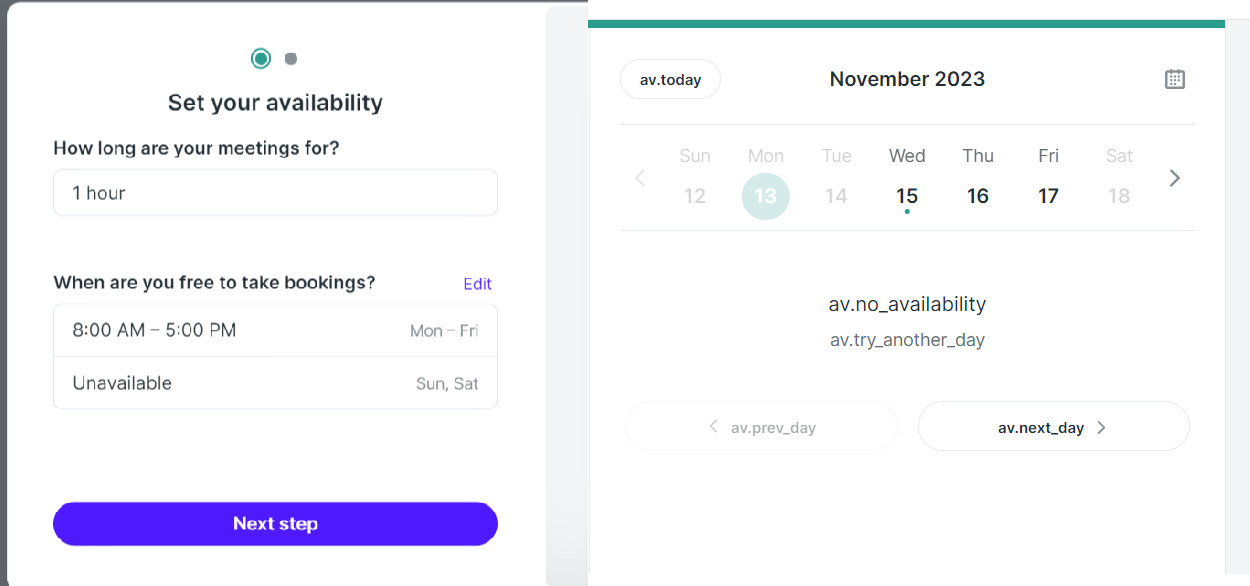
\includegraphics[scale=0.6]{slike/YouCanBookMe-Termin1.PNG} %veličina slike u odnosu na originalnu datoteku i pozicija slike
	\centering
	\caption{Primjer postavljanja dostupnih termina}
	\label{fig:promjene}
\end{figure}

U slučaju da se radi o klijentu koji odabire termin, on ima opciju izabrati samo neke od dostupnih termina. Nakon odabira ispunjava svoje podatke još jedanput kako bi organizator sastanka znao osnovne podatke o klijentu. U našem primjeru će na ovaj način funkcionirati pacijent uz iznimku da neće ponovno morati ispunjavati svoje podatke već će prilikom prijave za dostupni termin njegove osobne podatke moći vidjeti zdravstveni djelatnik. 

\begin{figure}[H]
	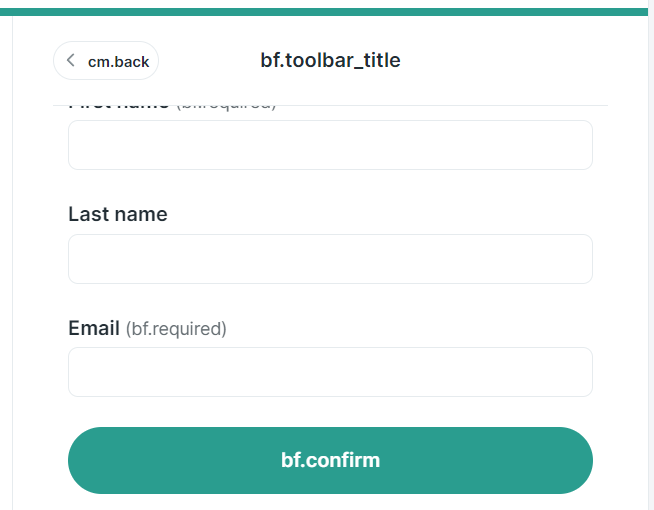
\includegraphics[scale=0.6]{slike/YouCanBookMe-Termin3.PNG} %veličina slike u odnosu na originalnu datoteku i pozicija slike
	\centering
	\caption{Primjer ispunjavanja podataka nakon odabira jednog od dostupnih termina}
	\label{fig:promjene}
\end{figure}

\textbf{\textit{Dodatno pojašnjenje}}\\

Korisnici sustava su:

\begin{packed_item}
	\item \textit{pacijenti}
	\item \textit{zdravstveni djelatnici}
	\item \textit{administrator}
\end{packed_item}

Svaki od te tri skupine korisnika ima različita dopuštenja. Djelatnici ustanove mogu vidjeti sve bolesnike i tretmane koji su im dodijeljeni. Nakon svakog obavljenog postupka djelatnik u sustav registrira pacijenta, a nakon završenog ciklusa oslobađa opremu. Pacijenti mogu vidjeti samo svoje tretmane. Administrator upravlja čitavim sustavom. Njemu su dostupni svi podaci i može definirati sve što je potrebno za ispravan rad sustava.

Za unesene podatke prilikom registracije u aplikaciju osigurat ćemo provjeru konzistentnosti s podacima iz baze podataka. Nakon toga korisnik postaje pacijent, izabire datum te ima mogućnost otkazati termin 1 dan prije početka tog termina.

Opreme, odnosno uređaji koje posjeduje ustanova se kategoriziraju. Spomenuli smo da slobodni termini ovise o ukupnom kapacitetu opreme/uređaja. Naravno da nije isto ako je čovjeku oštećena ruka ili noga. Tu se radi o drugoj opremi koju će zdravstveni djelatnik morati upotrijebiti za liječenja pacijenta. Dakle, korisnik kojemu je ozljeđena ruka neće zauzimati opremu korisniku kojemu je ozljeđena noga. Očekujemo da će broj oprema/uređaja za određeni dio tijela ipak biti veći od jedan, no svakako će biti ograničen.

Korisnik se u sustav prijavljuje upisivanjem korisničkog imena te svoje lozinke koja mora zadovoljavati određena pravila. Lozinka mora imati minimalno 8 znakova, od čega mora biti minimalno jedno veliko slovo te jedna znamenka. Ako korisnik prilikom registracije i smišljanja lozinke nije zadovoljio navedena pravila, dobit će upozorenje što mu nedostaje za ispravnu lozinku.

Aplikacija će imati obavezno početnu stranicu u kojoj će moći odabrati želi li se prijaviti ili registrirati u sustav. Zatim stranicu za prijavu i stranicu za registraciju. Na kraju je omogućen odlazak (nakon prijave korisnika s određenom ulogom) na povlaštenu stranicu za pacijente, zdravstvene djelatnike ili za administratore. \\

\textbf{\textit{Opseg projekta}}\\

Na projektu radi 7 osoba, studenata FER-a. Projekt se radi u edukativne svrhe provjere znanja studenata u sklopu predmeta "Programsko inženjerstvo". Vremensko ograničenje za prvu verziju projekta je 7 tjedana, a druga verzija (odnosno cijeli projekt) mora biti isporučen u roku od 14 tjedana od početka rada. Ukupan broj potrošenog vremena otići će najviše na sami rad oko projekta, ali značajan dio vremena otići će i na sastanke uživo gdje će tim redovito raspraviti o tjednom napretku.

\eject